% Copy figures and this snippet into your paper; requires graphicx.
\begin{figure}[t]
  \centering
  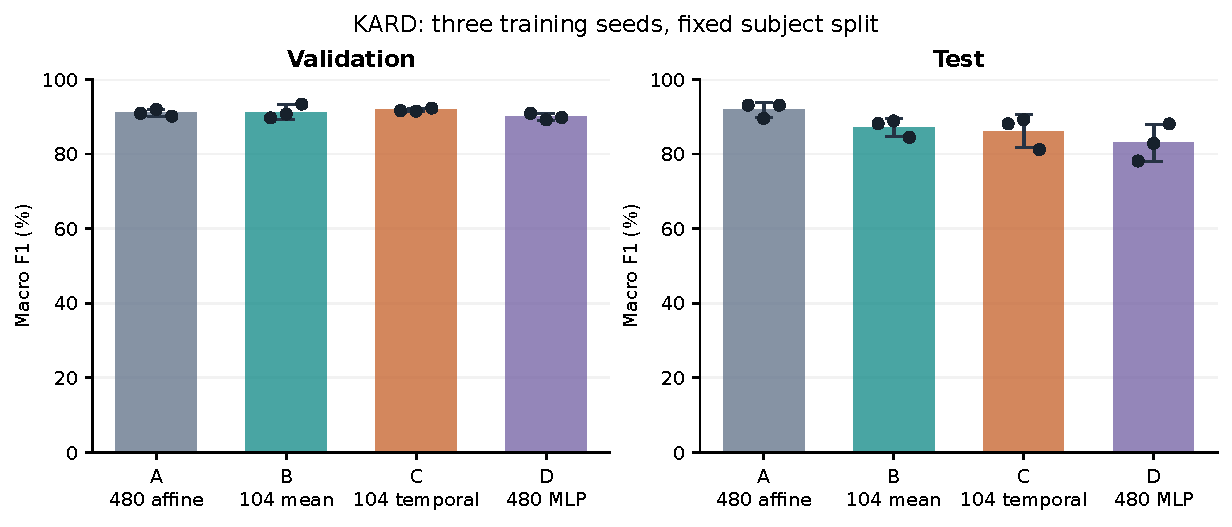
\includegraphics[width=\linewidth]{figures/macro_f1_comparison.pdf}
  \caption{KARD validation and descriptive test macro F1 for four prespecified
  frozen-feature controls. Points show three training seeds; error bars show
  sample standard deviation across training seeds on the same fixed subject
  split, not population confidence intervals.}
  \label{fig:kard-controlled-ablation}
\end{figure}
\begin{figure}[t]
  \centering
  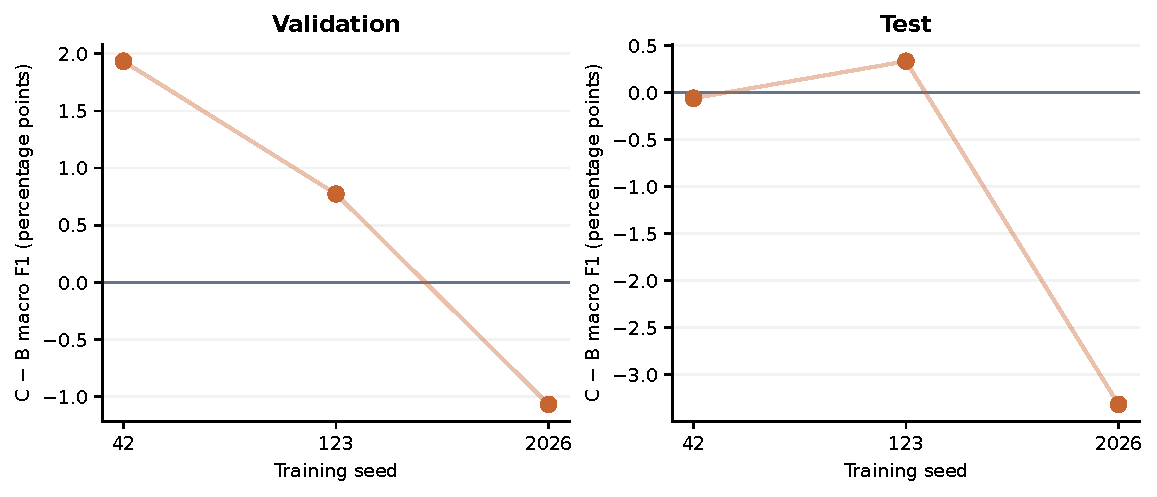
\includegraphics[width=\linewidth]{figures/paired_temporal_delta.pdf}
  \caption{Paired per-seed macro F1 changes when adding the causal depthwise
  temporal convolution to the otherwise identical compact model (C minus B).
  The previously observed test split is descriptive.}
  \label{fig:kard-temporal-paired}
\end{figure}
